\documentclass[12pt]{article}
\setlength{\oddsidemargin}{0in}
\setlength{\evensidemargin}{0in}
\setlength{\textwidth}{6.5in}
\setlength{\parindent}{0in}
\setlength{\parskip}{\baselineskip}

\usepackage{amsmath,amsfonts,amssymb,geometry}
\usepackage{graphicx}
\usepackage[all]{xy}
\usepackage{fancyhdr}
\usepackage{ulem}
\usepackage{adjustbox}
\usepackage[edges]{forest}
\pagestyle{fancy}
\setlength{\headheight}{15pt}

\begin{document}

CSCI 3104-300 Summer 2019 \hfill Problem Set 4 \\
Hoffman, Ryan \\
01/11

\hrulefill

\vspace{-3mm}
\begin{enumerate}

    \item (15 points) Shadow is writing a secret message to Harry and wants to prevent it from being understood by Thormund. 
    He decides to use Huffman encoding to encode the message. Magically, the symbol frequencies of the message are given by the 
    Lucas numbers, a famous sequence of integers discovered by the same person who discovered the Fibonacci numbers. 
    The nth Lucas number is defined as $L_n = L_{n-1} + L_{n-2}$ for $n > 1$ with base cases $L_0$ = 2 and $L_1$ = 1.
	\begin{enumerate}
    \item \label{q:huff:a} For an alphabet of $\Sigma=\{a,b,c,d,e,f,g,h\}$ with frequencies given by the first $|\Sigma|$ Lucas numbers, 
    give an optimal Huffman code and the corresponding encoding tree for Shadow to use.\par
    \textbf{Solution: (Next Page)}\par
    \begin{forest}
        [75 : abcdefgh
            [29 : h]
            [46 : abcdefg
                [18 : g]
                [28 : abcdef
                [11 : f]
                [17 : abcde
                [7 : e]
                [10 : abcd
                [4 : d]
                [6 : abc
                [3 : c]
                [3 : ab
                [1 : b]
                [2 : a]
                ]
                ]
                ]
                ]
                ]
            ]
        ]
    \end{forest}\par
    $$a:2 \quad b:1 \quad c:3 \quad d:4 \quad e:7 \quad f:11 \quad g:18 \quad h:29$$\par
    \newpage
    \item Generalize your answer to (\ref{q:huff:a}) and give the structure of an optimal code when the frequencies are the 
    first $n$ Lucas numbers.\par
    \textbf{Solution:}\par
        $$ \begin{array}{c|l} a & 1111111 \\ b & 1111110 \\ c & 111110 \\ d & 11110 \\ e & 1110 \\ f & 110 \\ g & 10 \\ h & 0 \end{array} $$

	\end{enumerate}

    \item (45 points) A good hash function $h(x)$ behaves in practice very close to the uniform hashing assumption analyzed in 
    class, but is a deterministic function. That is, $h(x)=k$ each time $x$ is used as an argument to $h()$. 
    Designing good hash functions is hard, and a bad hash function can cause a hash table to quickly exit the sparse loading 
    regime by overloading some buckets and under loading others. Good hash functions often rely on beautiful and complicated 
    insights from number theory, and have deep connections to pseudorandom number generators and cryptographic functions. 
    In practice, most hash functions are moderate to poor approximations of uniform hashing.
	
    \smallskip Consider the following hash function. Let $U$ be the universe of strings composed of the characters from the 
    alphabet $\Sigma=[${\tt A}$,\dots,${\tt Z}$]$, and let the function $f(x_{i})$ return the index of a letter $x_{i}\in \Sigma$, 
    e.g., $f(${\tt A}$)=1$ and $f(${\tt Z}$)=26$. Finally, for an $m$-character string $x\in \Sigma^{m}$, define $h(x) = \left(\left[\sum_{i=1}^{m}f(x_{i})\right]\!\! \mod \ell\right)$, 
    where $\ell$ is the number of buckets in the hash table. That is, our hash function sums up the index values of the characters 
    of a string $x$ and maps that value onto one of the $\ell$ buckets.
	
	\begin{enumerate}
    	\item The following list contains US Census derived last names: \\
    	{\tt http://www2.census.gov/topics/genealogy/1990surnames/dist.all.last} \\
        Using these names as input strings, first choose a uniformly random 50\% of these name strings and then hash them 
        using $h(x)$.
    	
        Produce a histogram showing the corresponding distribution of hash locations when $\ell=200$. Label the axes of your 
        figure. Briefly describe what the figure shows about $h(x)$, and justify your results in terms of the behavior of $h(x)$. 
        Do not forget to append your code.\par
        {\footnotesize Hint: the raw file includes information other than name strings, which will need to be removed; and, think 
        about how you can count hash locations without building or using a real hash table.}\par
        \textbf{Solution:}\par
        \begin{figure}[h!]
            \centering
            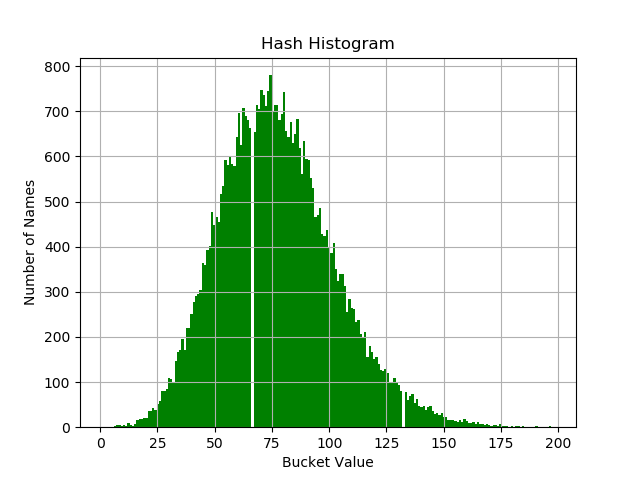
\includegraphics{PS4_Histo.png}
            \caption{Hashing}
        \end{figure}
            Here, in our figure, we see that the distribution of hash locations when the number of buckets, $\ell=200$, is in the form of a bell curve.
            I have no further understanding of what is happening beyond that. \par
        \newpage
    	\item Enumerate at least 4 reasons why $h(x)$ is a bad hash function relative to the ideal behavior of uniform hashing.\par
        \textbf{Solution:}\par
            \begin{itemize}
                \item $h(x)$ is a bad hash function because the assumption of simple uniform hashing is that any given key
                is equally likely to hash in to any of the buckets independently of where any other key has hashed to.
                \item $h(x)$ is a bad hash function because a good hash function would minimize the chance of having character strings
                such as \textit(the) and \textit(then) occuring in the same bucket.  
                \item $h(x)$ is a bad hash function because a good hash function derives the key that assumes an independent relationship
                with any potential patterns found in the data.
                \item $h(x)$ is a bad hash function because there could be a need to have keys that more closely related yield results of 
                hash values that are farther apart. (i.e. for linear probing) 
            \end{itemize}
        \item Produce a plot showing (i) the length of the longest chain (were we to use chaining for resolving collisions 
        under $h(x)$) as a function of the number $n$ of these strings that we hash into a table with $\ell=200$ buckets, 
        (ii) the exact upper bound on the depth of a red-black tree with $n$ items stored, and (iii) the length of the longest 
        chain were we to use a uniform hash instead of $h(x)$. Include a guide of $c\,n$ \par
    	
        Then, comment (i) on how much shorter the longest chain would be under a uniform hash than under $h(x)$, and (ii) on 
        the value of $n$ at which the red-black tree becomes a more efficient data structure than $h(x)$ and separately a uniform 
        hash.\par
        \textbf{Solution: (Next Page)}\par
        \newpage
        \begin{figure}[!h]
            \centering
            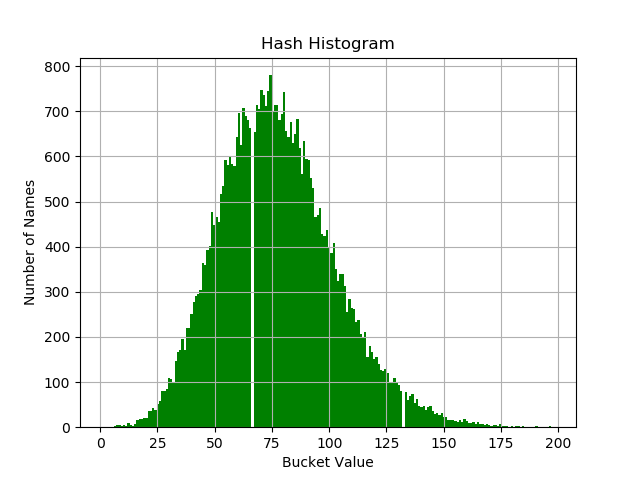
\includegraphics{PS4_Histo.png}
            \caption{Hashing}
        \end{figure}
            (i) The image for this plot is exactly the same because collision resolution with chaining simply involves storing the repeat 
            values in a linked list. Therefore I have no idea what the length of the longest chain would be or how much shorter it would be 
            under uniform hashing. My guess is that it would be much shorter because this h(x) is bad in comparison as described above.\par
            (ii) I'm really not sure why we're talking about red-black trees so it's difficult to understand what to write. The exact upper
            bound on a red-black tree is, according to CLRS, "Lemma 13.1
            A red-black tree with $n$ internal nodes has height at most $2lg(n+1)$." \par

	\end{enumerate}

	\newpage
	\item (20 points) Grog is struggling with the problem of making change for $n$ cents using the smallest number of coins for his purchase of a new great sword. Grog has coin values of $v_{1}<v_{2}<\dots<v_{r}$ for $r$ coin types, where each coin's value $v_{i}$ is a positive integer. His goal is to obtain a set of counts $\{d_{i}\}$, one for each coin type, such that $\sum_{i=1}^{r}d_{i}=k$ and where $k$ is minimized.
	\begin{enumerate}
	\item A greedy algorithm for making change is the \textbf{cashier's algorithm}, which all young wizards learn. Harry writes the following pseudocode on the whiteboard to illustrate it, where $n$ is the amount of money to make change for and $v$ is a vector of the coin denominations:
	%
	\begin{small}
	\begin{verbatim}
	wizardChange(n,v,r) :
	   d[1 .. r] = 0       // initial histogram of coin types in solution
	   while n > 0 {
	      k = 1
	      while ( k < r and v[k] > n ) { k++ }
	      if k==r { return 'no solution' }
	      else { n = n - v[k] }
	   }
	   return d
	\end{verbatim}
	\end{small}
    Thormund snorts and says Harry's code has bugs. Identify the bugs and explain why each would cause the algorithm to fail.\par
    \textbf{Solution:}\par
        I have no idea what bugs there are but here are a few things that stick out:\par
        \begin{itemize}
            \item Not sure what the "d[1 .. r] = 0" is for because we're not told what $r$ is.
            \item It looks like the while loop just keeps incrementing k until either $k>r$ or $v[k]<n$ 
        \end{itemize}
	\item Sometimes the dwarves at Rocky Mountain Bank run out of coins,%
	%
	\footnote{It's a little known secret, but dwarven pets like to \textit{eat} the coins. It isn't pretty for the coins, in the end.}
	%
    and make change using whatever is left on hand. Identify a set of U.S. coin denominations for which the greedy algorithm does not 
    yield an optimal solution. Justify your answer in terms of optimal substructure and the greedy-choice property. 
    (The set should include a penny so that there is a solution for every value of $n$.)\par
    \textbf{Solution: (Next Page)}\par
    \newpage
	1. Greedy-choice property: A global optimum can be arrived at by selecting a local optimum.\par
    2. Optimal substructure: An optimal solution to the problem contains an optimal solution to subproblems.
    Using the following U.S. coin denominations:\par

    \begin{tabular}{ c c c }
        Penny & Dime & Quarter \\
        1  & 10  & 25 \\
      \end{tabular}\par
    Now, given our greedy algorithm, when $n=30$ cents, our solution will yield five (5) pennies and one (1) quarter. 
    This is six (6) coins but we can see that three (3) dimes would be a better (optimal, in fact) solution.\par

    \item On the advice of wizards specializing in electricity, Rocky Mountain Bank has announced that they will be changing all  
    coin denominations into a new set of coins denominated in powers of $c$, i.e., denominations of $c^{0}, c^{1}, \dots , c^{\ell}$ 
    for some integers $c>1$ and $\ell\geq 1$.  (This will be done by a spell that will magically transmute old coins into new coins, before your very eyes.) 
    Prove that the cashier's algorithm will always yield an optimal solution in this case.
	
    Hint: first consider the special case of $c=2$.\par
    \textbf{Solution:}\par
      Using CLRS as a guide, to prove the Cashier's algorithm will always yield an optimal solution in the above case, we need to start with
      a proof of the following Lemma:\par
      For $i = 0, 1, ...,k$ let $d_i$ be the number of coins of denomination $c^i$ used in an optimal solution to making change for $n$ cents.
      Then for $i = 0,1,...,k-1$, we have $d_i < c$.\par
      Proof by Contradiction:\par
      I still cannot figure out how this works. I know that we show a non-greedy algorithm will always fail to 
      provide an optimal solution and that's somehow a contradiction to what we want which serves as proof
      but that doesn't seem like it proves anything at all. 
	\end{enumerate}
    \newpage
    \item (20 points) We saw in the previous problem that the cashier's (greedy) algorithm for making change doesn't handle 
    arbitrary denominations optimally. In this problem you'll develop a dynamic programming solution which does, but with a 
    slight twist. Suppose we have at our disposal an arbitrary number of \emph{cursed} coins of each denomination 
    $d_1, d_2, \dotsc, d_k$, with $d_1 < d_2 < \dotsc < d_k$, and we need to provide $n$ cents in change. We will always 
    have $d_1=1$, so that we are assured we can make change for any value of $n$. The curse on the coins is that in any one 
    exchange between people, with the exception of $i=2$, if coins of denomination $d_i$ are used, then coins of 
    denomination $d_{i-1}$ \emph{cannot} be used. Our goal is to make change using the minimal number of these cursed 
    coins (in a single exchange, i.e., the curse applies).\par

    \begin{enumerate}
        \item For $i \in \{1,\dotsc,k\}$, $n \in \mathbb{N}$, and $b \in \{0,1\}$, let $C(i,n,b)$ denote the number of 
        cursed coins needed to make $n$ cents in change using only the first $i$ denominations $d_1, d_2, \dotsc, d_i$, where 
        $d_{i-1}$ is allowed to be used if and only if $i \leq 2$ or $b=0$. That is, $b$ is a Boolean ``flag'' variable 
        indicating whether we are excluding denomination $d_{i-1}$ or not ($b=1$ means exclude it). 	
        Write down a recurrence relation for $C$ and prove it is correct. Be sure to include the base case.\par
        \textbf{Solution:}\par
        No solution at this time.
        \item Based on your recurrence relation, describe the order in which a dynamic programming table for $C(i,n,b)$ 
        should be filled in.\par
        \textbf{Solution:}\par
        No solution at this time.
        \item Based on your description in part (b), write down pseudocode for a dynamic programming solution to this problem, 
        and give a $\Theta$ bound on its running time (remember, this requires proving both an upper \emph{and} a lower bound).\par
        \textbf{Solution:}\par
        No solution at this time.
    \end{enumerate}

\end{enumerate}

\end{document}


